\documentclass[xcolor=pdftex,dvipsnames,table,aspectratio=169]{beamer}
%\documentclass[xcolor=pdftex,dvipsnames,table,handout,aspectratio=169]{beamer}

%\setbeameroption{show notes}

\usepackage{bm,graphicx,multirow,amsmath,tikz} %fancybox,
\usepackage{color}%,textpos}
\usepackage[round]{natbib}
\usepackage[normalem]{ulem}
\usepackage{hyperref}
\usepackage{lastpage}
\usepackage{array}
\usepackage{color}
\usepackage{framed}
\usepackage{hyperref}

% Define Western colours
\definecolor{western}{rgb}{.306,.152,.524}
\definecolor{westerngray}{rgb}{.512,.508,.524}

%% Define BEAMER colours
\setbeamercolor{frametitle}{bg=western,fg=white}
\setbeamercolor{framesubtitle}{bg=western,fg=black}
\setbeamercolor{title}{fg=white,bg=western}
\setbeamercolor{author}{fg=white,bg=western}
\setbeamercolor{institute}{fg=white,bg=western}
\setbeamercolor{date}{fg=white,bg=western}

%% Set BEAMER fonts
\setbeamerfont{title}{shape=\bf}
\setbeamerfont{frametitle}{shape=\sc,size=\Large}
\setbeamerfont{framesubtitle}{shape=\sc,size=\Large}
\setbeamerfont{footline}{shape=\sc}

%% Define BEAMER toc
\setbeamercolor{section in toc}{fg=western}
\setbeamercolor{subsection in toc}{fg=westerngray}
\setbeamertemplate{sections/subsections in toc}[ball]

%% Define BEAMER background
\setbeamercolor{background canvas}{bg=white}

%% Define BEAMER footer
\setbeamertemplate{navigation symbols}{}
\setbeamercolor{footline}{fg=white,bg=western}
\setbeamertemplate{footline}{%
  \begin{beamercolorbox}[wd=\paperwidth]{footline}
    \vskip5pt

    \raisebox{.05in}{
      \scriptsize{\bf \insertshorttitle}
    }
    \hfill
    \raisebox{.05in}{
      \scriptsize{\bf \insertframenumber/\inserttotalframenumber} 
    }
    \hspace{5pt}

    \vskip5pt
  \end{beamercolorbox}
}

%% Define BLOCK environment
\setbeamercolor{block title}{fg=western}
\setbeamerfont{block title}{series=\bfseries}

%% Define ENUMERATE and ITEMIZE environements
\setbeamertemplate{itemize item}[ball]
\setbeamertemplate{enumerate item}[ball]
\setbeamercolor{item projected}{bg=western}

%% Define BEAMER toc
\setbeamercolor{sections/subsections in toc}{fg=blue!75}
\setbeamertemplate{sections/subsections in toc}[ball]

% %% Define SECTION openings
% \AtBeginSection[]{
%   \begin{frame}{\insertshorttitle}
%     \tableofcontents[currentsection,subsectionstyle=hide/hide/hide]
    
%   \end{frame}
% }

%% Define BEAMER frametitle
\addtobeamertemplate{frametitle}{
   \let\insertframetitle\insertsectionhead}{}
\addtobeamertemplate{frametitle}{
   \let\insertframesubtitle\insertsubsectionhead}{}


\makeatletter
  \CheckCommand*\beamer@checkframetitle{\@ifnextchar\bgroup\beamer@inlineframetitle{}}
  \renewcommand*\beamer@checkframetitle{\global\let\beamer@frametitle\relax\@ifnextchar\bgroup\beamer@inlineframetitle{}}
\makeatother

% Define counters for example and exercise
\newcounter{example}
\newcounter{exercise}

% Define example and exercise commands
\renewcommand{\example}
{\stepcounter{example}Example \lecturenum.\arabic{example}}
\newcommand{\examplectd}
{Example \lecturenum.\arabic{example}\ ctd}
\newcommand{\exercise}
{\stepcounter{exercise}Exercise \lecturenum.\arabic{exercise}}
\newcommand{\exercisectd}
{Exercise \lecturenum.\arabic{exercise}\ ctd}

\newcommand{\lecturenum}{18}

\title[SS2857]{Probability and Statistics I}
\subtitle{\lecturenum. Chapter 4 Summary Exercise}

\date{}

%% Add logo
% \titlegraphic{\includegraphics[height=2cm]{../uwo_logo_reversed}}

%% Initialize R



\begin{document}

{
\setbeamertemplate{footline}{}
\setbeamercolor{background canvas}{bg=western}

\begin{frame}
  \addtocounter{framenumber}{-1}

  \maketitle
\end{frame}
}

\begin{frame}

\begin{block}{How far do Western students live from campus?}

Use Google Maps to compute the distance from your home to campus. Enter the result in the spreadsheet at:
\begin{center}
\url{https://uwoca-my.sharepoint.com/:x:/g/personal/sbonner6_uwo_ca/Ee9EAgVPP2pJkSgS7SPQCZoBhubeOhoSTgMd-2QrGf9KIg?e=o27rxM}
\end{center}
\end{block}
\end{frame}




\begin{frame}
\begin{block}{How far do Western students live from campus?}
\begin{center}
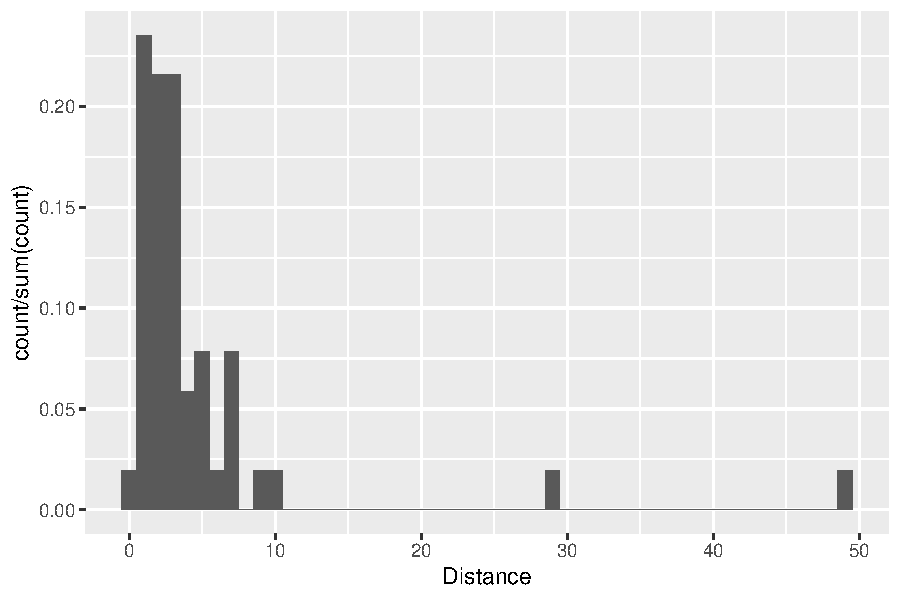
\includegraphics[height=.7\textheight]{figure/histogram-1.pdf}
\end{center}
\end{block}
\end{frame}

\begin{frame}
\begin{block}{How far do Western students live from campus?}
\begin{center}
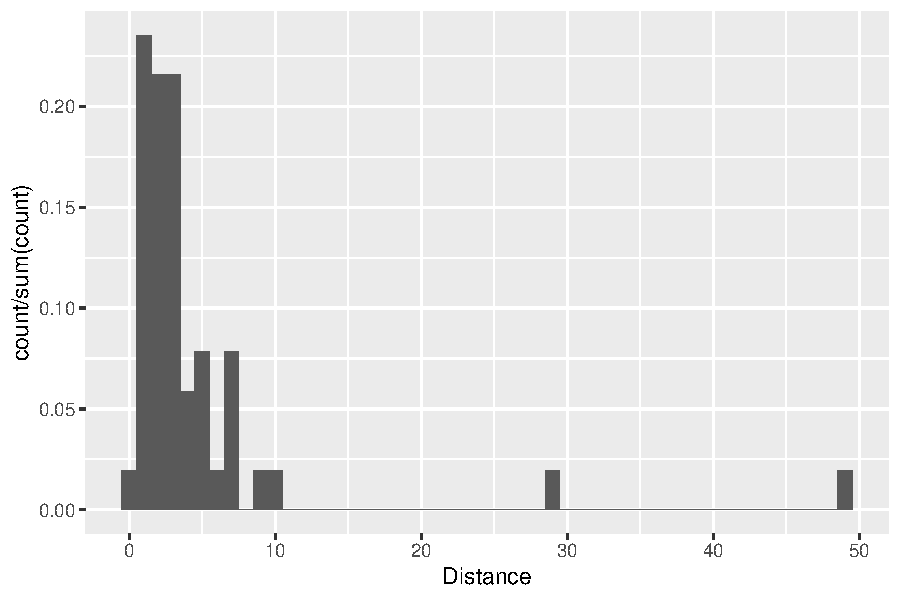
\includegraphics[height=.5\textheight]{figure/histogram-1.pdf}
\end{center}

$$
n=51,\quad
\hat \mu = 4.634,\quad
\widehat{\sigma^2} = 58.011 
$$
\end{block}
\end{frame}

\begin{frame}


\begin{block}{How far do Western students live from campus?}
Use the data summaries on the previous slide to estimate the parameters assuming:
\begin{itemize}
\item the distribution is normal.
\item the distribution is gamma.
\end{itemize}
\end{block}
For each distribution find:
\begin{enumerate}
\item The value $d_1$ so that 97.5\% of students live less than $d_1$~km from campus.
\item The value $d_2$ so that 97.5\% of students live greater than $d_2$~km from campus.
\end{enumerate}

\begin{center}
Which distribution do you believe will fit the data better?
\end{center}
\end{frame}


\begin{frame}

\begin{block}{Normal Distribution}
$$
\hat \mu = 4.634, \quad \widehat{\sigma^2} = 58.011 
$$

\begin{center}
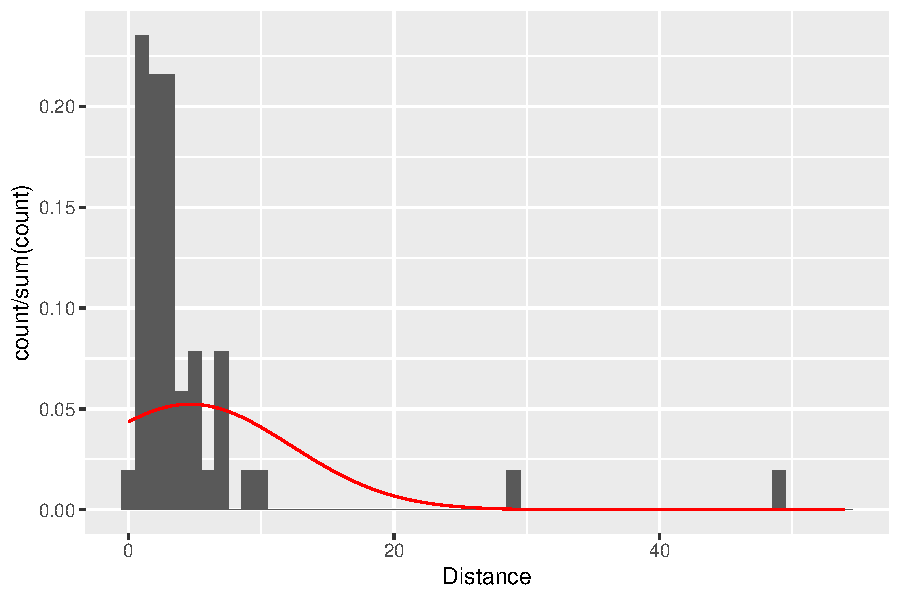
\includegraphics[height=.5\textheight]{figure/normal-1.pdf}
\end{center}

\end{block}
\end{frame}



\begin{frame}

\begin{block}{Gamma Distribution}
$$
\hat{\alpha} = 0.37, \quad \hat{\beta} = 12.519 
$$

\begin{center}
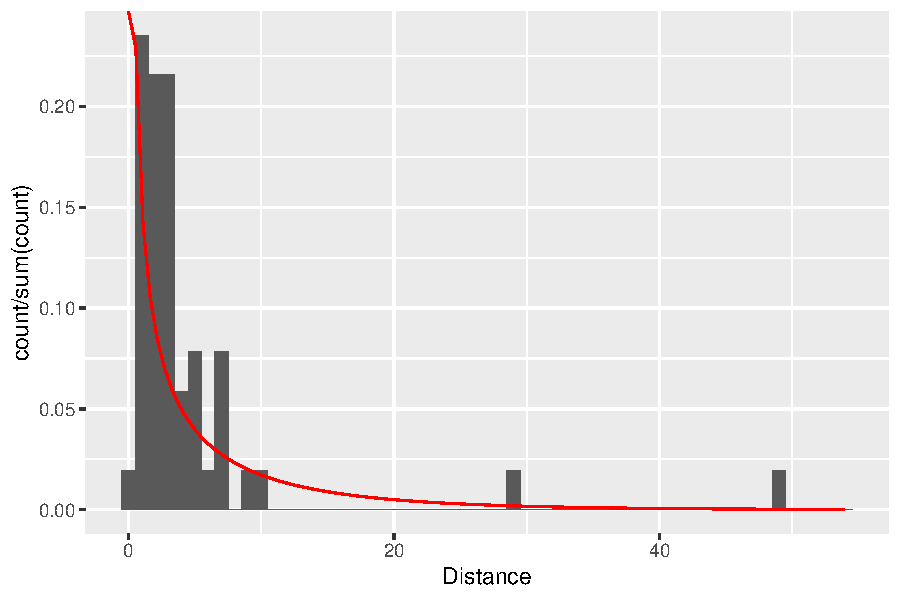
\includegraphics[height=.5\textheight]{figure/gamma-1.pdf}
\end{center}
\end{block}
\end{frame}

\begin{frame}

\begin{block}{Percentile Plots}

Suppose that the data come from a distribution with percentiles $\eta_p$. Then we would expect the $k$-th largest data point to be close to $\eta_{(k-.5)/n}$\footnote{The extra $-.5$ keeps us below 100\%.}. 

\bigskip

With 51 observations, we would expect
\begin{itemize}
\item the smallest observation to be close to $\eta_{\frac{.5}{51}}$
\item the next smallest observation to be close to $\eta_{\frac{1.5}{51}}$
\item $\cdots$
\item the biggest observation to be close to $\eta_{\frac{50.5}{51}}$
\end{itemize}

\bigskip

Generally, if $x_{(1)},\ldots,x_{(n)}$ represent the \textit{ordered} data then
$$
x_{(k)}\approx \eta_{\frac{k}{n}}.
$$

\bigskip

A percentile plot plots $x_{(k)}$ vs $\eta_{\frac{k}{n}}$ for $k=1,\ldots,n$. If the data were generated from that distribution then the points will lie close to a straight line.
\end{block}
\end{frame}

\begin{frame}

\begin{block}{Percentile Plots}

Suppose that the data come from a distribution with percentiles $\eta_p$. Then we would expect the $k$-th largest data point to be close to $\eta_{(k-.5)/n}$\footnote{The extra $-.5$ keeps us below 100\%.}. 

\bigskip

Generally, if $x_{(1)},\ldots,x_{(n)}$ represent the \textit{ordered} data then
$$
x_{(k)}\approx \eta_{\frac{k}{n}}.
$$

\bigskip

A percentile plot plots $x_{(k)}$ vs $\eta_{\frac{k}{n}}$ for $k=1,\ldots,n$. If the data were generated from that distribution then the points will lie close to a straight line.
\end{block}
\end{frame}




\begin{frame}

\begin{block}{Percentile Plots -- Normal}

\begin{center}
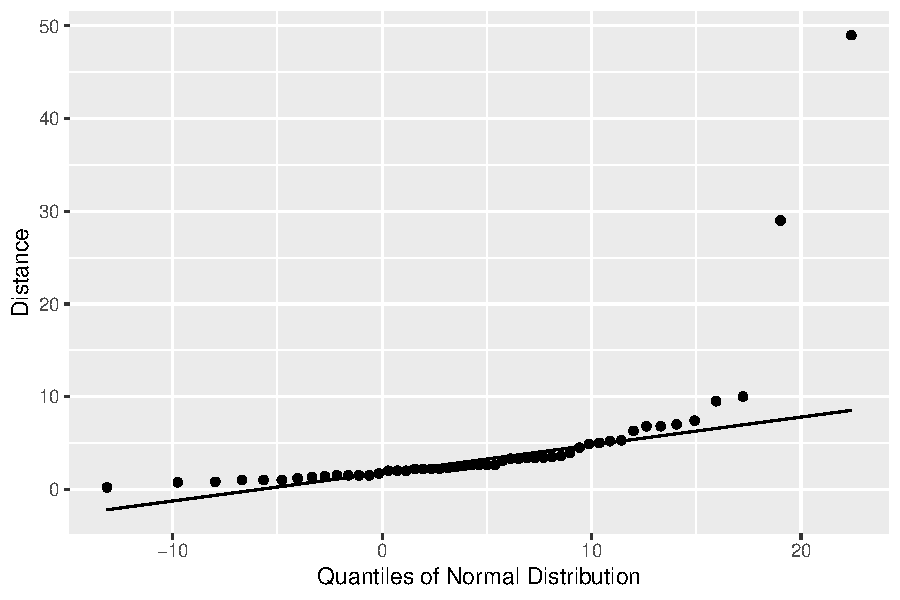
\includegraphics[height=.7\textheight]{figure/qqnorm-1.pdf}
\end{center}

\end{block}
\end{frame}




\begin{frame}

\begin{block}{Percentile Plots -- Gamma}

\begin{center}
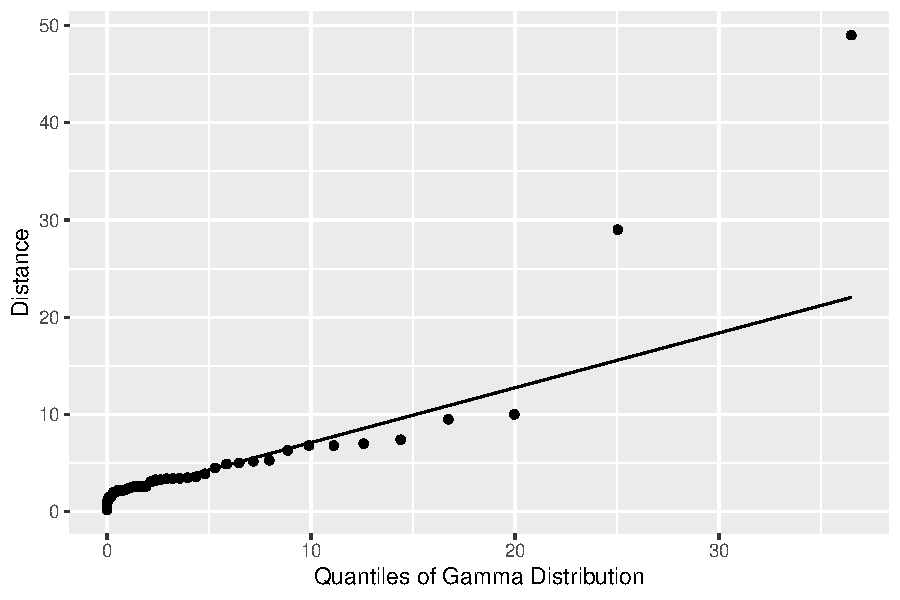
\includegraphics[height=.7\textheight]{figure/qqgamma-1.pdf}
\end{center}

\end{block}
\end{frame}

\end{document}


